\documentclass[12pt,a4paper]{./../../template/memoire-umons}

\usepackage{xspace}
\usepackage{lmodern}
\usepackage[babel=true]{microtype}

\usepackage[latin1]{inputenc}
\usepackage[T1]{fontenc}
\usepackage[francais]{babel}
\usepackage{amssymb,amsmath,amsthm}
%\usepackage{hyperref}% hyperliens dans le PDF, pas pour impression

\usepackage{algorithm}
\usepackage{algpseudocode}
\usepackage{tikz}
\usetikzlibrary{arrows,shapes,positioning}
\usetikzlibrary{decorations.markings}



\usepackage{hyperref}



\usepackage{amsmath}




\title{Algorithmes probabilistes de localisation impl�ment�s sur une brique EV3}
\author{Beno\^it \textsc{Hofbauer}}
\date{2014--2015}
%\directeur{Hadrien Melot}
\directeurs{Hadrien M\'elot\\ Pierre Hauweele}
%\codirecteurs{Pierre Hauweele}
\service{Algorithmique}

\discipline{informatiques}

%%%%%%%%%%%%%%%%%%%%%%%%%%%%%%%%%%%%%%%%%%%%%%%%%%%%%%%%%%%%%%%%%%%%%%%%
%% Vos macros
\newcommand{\source}[1]{     \textbf{Source:} {#1} }

%%%%%%%%%%%%%%%%%%%%%%%%%%%%%%%%%%%%%%%%%%%%%%%%%%%%%%%%%%%%%%%%%%%%%%%%

% Compile uniquement certains morceaux sans perdre les références
% automatiques et la table des matières des parties déjà compilées :
%\includeonly{introduction,chapitre1}

\begin{document}
% Éventuellement utiliser l'environnement « preface » pour avoir une
% numérotation des pages en chiffres romains.
\begin{preface}
\section*{Remerciements}
Je tiens � remercier Hadrien M�lot le directeur de ce m�moire et Pierre Hauweele le codirecteur de ce m�moire pour m'avoir apport� leur expertise dans le domaine et leur aide pr�cieuse.

Je tiens �galement � remercier ma m�re qui m'a aid� � relire et structurer ce document.
\section*{R�sum�}
L'objectif de ce m�moire est de d�velopper des aspects th�oriques de la robotique en y liant une validation pratique. La localisation d'un robot dans son environnement est le principal sujet abord�. Les algorithmes de localisation probabilistes, Extended Kalman filter (EKF) ainsi que Monte Carlo localization (MCL) seront �tudi�s en profondeur. Toutefois, une multitude de sous-sujets en d�coulent, tels que la caract�risation des capteurs et des actuateurs, les syst�mes d'exploitation dans la robotique, l'analyse d'images...

Le kit EV3 de Lego est utilis� pour la validation pratique des concepts th�oriques pr�sent�s. Ce kit est compos� d'une brique intelligente, de capteurs, de moteurs ainsi que d'�l�ments de construction qui permettent de r�aliser rapidement la structure d'un robot. Ce kit est combin� avec un smartphone tournant sous Android. Ce smartphone permet d'ajouter de la puissance de calcul et de se servir des capteurs pr�sents sur le smartphone. En effet, les smartphones actuels poss�dent un grand nombre de capteurs � couts r�duits et leur capacit� de calcul est importante.
\section*{Avant-propos}
Les deux mots � voiture autonome � sont sur les l�vres de tous les constructeurs automobiles depuis quelques ann�es. Plusieurs prototypes ont �t� r�alis�s depuis les ann�es 1980\cite{Stentz_1985_1234}\cite{Kanade:1986:ALV:324634.325197}. Cependant, ces prototypes �taient limit�s soit par la vitesse du v�hicule soit par les restrictions de l'environnement dans lequel ils �voluaient. L'�volution des technologies li�es aux capteurs et l'augmentation de la puissance des processeurs ont permis une avanc�e consid�rable dans le domaine. Google, annonce en octobre 2010 \cite{NYT2010} avoir con�u un syst�me de pilotage automatique pour automobile. Ce prototype est capable de se d�placer dans la circulation automobile sans assistance humaine. � ce jour, de nombreux constructeurs automobiles travaillent sur des voitures autonomes. On peut citer Audi, Toyota\cite{ToyotaBot}, Nissan\cite{bbc2013}, Mercedes-Benz.

La multitude de capteurs qui �quipent ces v�hicules est �videmment primordiale. Toutefois, sans traitement et croisement de ces mesures, il est impossible de d�velopper un v�hicule autonome. Pour cela, des algorithmes ont �t� d�velopp�s. Ces algorithmes permettent aux v�hicules de se localiser dans leur environnement pour ensuite �tablir leur parcours. Ces algorithmes doivent prendre en compte que les valeurs des capteurs peuvent �tre entach�es d'erreurs. Ils doivent �galement prendre en compte que les capteurs ne permettent de capter qu'une partie de l'environnement du v�hicule.
Des v�hicules comme la voiture autonome de Google embarquent un grand nombre des capteurs de hautes pr�cisions. Toutefois, �quiper des voitures de ces capteurs se r�v�le encore tr�s on�reux. Il est donc int�ressant de se demander quelles sont les limites des algorithmes de localisation avec des capteurs � faibles couts. Ces algorithmes sont-ils perfectibles ? Les robots de nettoyage domestique\cite{futura-sciences} sont des exemples de robots qui ont des capteurs simples et peu on�reux, mais qui doivent se d�placer dans un environnement complexe.   

Le livre de Sebastian Thrun � Probabilistic Robotics � \cite{Thrun:2005:PR:1121596} qui est la bible dans le domaine de la robotique a �t� une ressource importante pour la r�daction de ce m�moire. Rappelons que Sebastian Thrun est l'ing�nieur principal qui a lanc� le projet � Google driverless car �. Le m�moire de Pierre Hauweele \cite{Hauweele:2013} donne certaines d�monstrations th�oriques plus en profondeur alors que ce m�moire est plus centr� sur les aspects pratiques.

\tableofcontents
\listoffigures
\end{preface}




%\include{introduction}
\part{Localisation d'un robot dans son environnement }



\chapter{Probl�me de localisation}
\section{Explication du probl�me}
Le probl�me de localisation d'un robot mobile consiste � d�terminer sa position � un instant donn� sur une carte donn�e. Pour atteindre cet objectif, le robot a � sa disposition les mouvements qu'il a r�alis�s, des mesures provenant de ses capteurs ainsi qu'une carte de son environnement. 

Cette situation peut facilement �tre compar�e � un promeneur cherchant sa position dans la nature avec une carte topographique. Cette personne n'a � sa disposition que les observations qu'elle peut r�aliser (sans l'aide d'instrument de localisation comme un GPS). Elle peut se localiser � l'aide des montagnes qui sont des points de rep�re int�ressants. Elle peut �galement essayer de trouver des ressemblances avec le chemin qu'elle parcourt et ce qu'elle peut observer sur la carte. Cependant, il est difficile d'estimer exactement la distance qui s�pare cette personne de la montagne. La distance parcourue par cette personne entre deux points est �galement difficile � estimer sans erreur.  Toutes ces informations sont donc approximatives.
Malgr� ces erreurs d'approximations, gr�ce � la quantit� d'informations accumul�es durant son parcours cette personne a de fortes chances d'�tre de plus en plus certaine de sa position. En effet, en d�but de parcours, cette personne peut supposer �tre � un ensemble d'endroits diff�rents � la suite d'un manque d'informations en sa possession. Par la suite gr�ce aux nouvelles informations elle peut proc�der par �limination pour d�terminer sa position.

Il s'av�re que les robots doivent faire face aux m�mes types de probl�mes pour se localiser. Gr�ce � l'odom�trie, il est possible de d�terminer les mouvements du robot en fonction de la rotation de chacun des moteurs du robot. � l'aide de capteurs tels que les capteurs infrarouges, il est possible de d�terminer la distance entre la position du robot et un objet. Cependant comme pour le promeneur ces informations sont entach�es d'erreurs de pr�cisions. De plus, dans le cas des capteurs de distance infrarouges ou ultrasoniques, les ondes peuvent �tre r�fl�chies de fa�on inattendue selon la forme et la mati�re de la surface de l'objet r�fl�chissant l'onde. Une solution na�ve serait de vouloir acheter des d�tecteurs et des moteurs toujours plus pr�cis. Cependant, le cout des capteurs plus pr�cis est plus important. De plus, des erreurs peuvent �tre impossibles � g�rer � l'aide de mat�riel plus pr�cis. En effet, il peut arriver que les roues du robot n'adh�rent pas parfaitement � la route. Ce qui entraine le glissement des roues et donc bien que le robot reste immobile, les moteurs enregistreront un mouvement. Finalement, les capteurs ont �galement des limitations physiques, il est par exemple impossible pour une cam�ra de voir � travers les murs.  

La pr�dictibilit� de l'environnement est un �l�ment important dans le choix d'appliquer ou non des algorithmes probabilistes. Dans le cas d'un environnement bien structur� comme une chaine de montage, le degr� de pr�dictibilit� est bien plus important que lorsque le robot �volue en ville ou dans une maison. L'impr�dictibilit� augmente fortement lorsque le robot �volue dans un environnement en pr�sence de personnes. Les algorithmes probabilistes permettent de pallier � l'impr�dictibilit� d'un environnement. 


\section{D�finition formelle du probl�me}
\subsection{Mod�le de mouvement et d'observation}

L'objectif de la localisation d'un robot est de d�finir sur une carte la position du robot � un instant donn�. Cette position est d�not�e par le vecteur $x_t$. 
Dans la suite de ce m�moire, la position du robot est d�finie par ses coordonn�es dans un espace � deux dimensions ainsi que par son orientation. Les algorithmes pr�sent�s ne se limitent pas � cette situation et peuvent �tre utilis�s pour un espace � un nombre de dimensions sup�rieures. L'�tat des bras des robots industriels\cite{osha.gov} peut �galement �tre repr�sent� � l'aide de l'angle de chaque articulation du bras. Toutefois, les principes sont plus simples � comprendre dans cette situation et cette situation est souvent suffisante pour les robots mobiles. Formellement, la position d'un robot dans un espace � deux dimensions peut-�tre d�finit par le vecteur :
$$ x_t = \begin{pmatrix} x \\ y \\ \theta \end{pmatrix}$$

o� $x, y$ correspondent aux coordonn�es dans un espace � deux dimensions et $\theta$ correspond � l'orientation du robot (voir ~\ref{PR2D}). 


\begin{figure}
\begin{center}
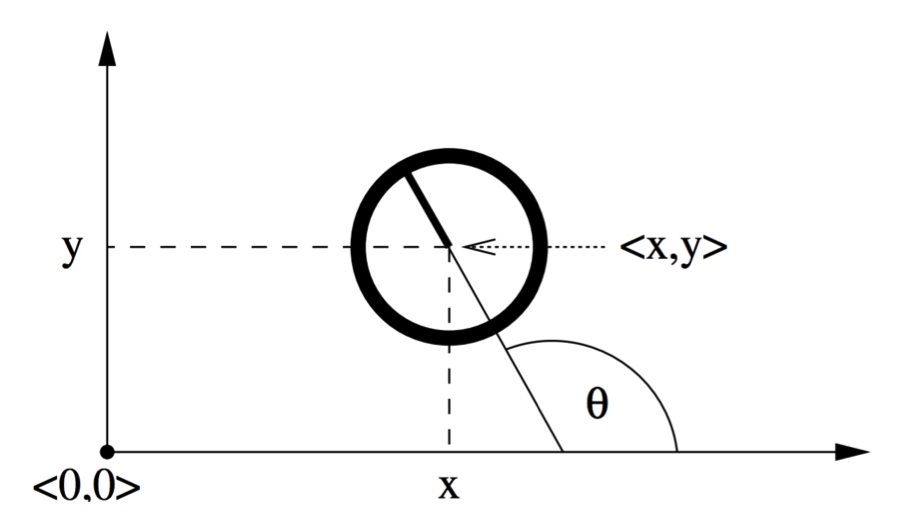
\includegraphics[scale=0.7]{./../img/PositionRobot.png}
\caption{Position d'un robot dans un espace � deux dimensions }
\source{Probabilistic Robotics\cite{Thrun:2005:PR:1121596}}
\end{center}

\label{PR2D}
\end{figure}

Pour d�terminer la position du robot dans le temps, il faut prendre en consid�ration les contr�les du robot (not�s : $u_t$) ainsi que les observations effectu�es par le robot (not�es : $z_t$). Les algorithmes qui seront pr�sent�s par suite suivent l'hypoth�se de Markov. C'est-�-dire que l'�tat $x_{t}$ ne d�pend que de l'�tat $x_{t-1}$ ainsi que des contr�les $u_{t}$ et des observations courantes $z_{t}$(voir figure ~\ref{HM}). 


\begin{figure}
\begin{center}
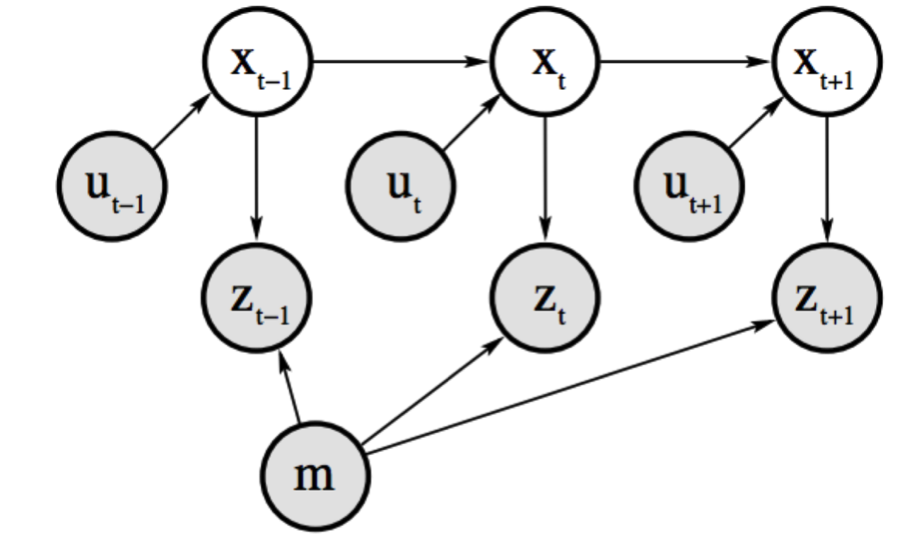
\includegraphics[scale=0.7]{./../img/HypotheseMarkov.png}
\caption{Hypoth�se de Markov permettant de d�terminer la position actuelle du robot}
\source{Probabilistic Robotics\cite{Thrun:2005:PR:1121596}}
\end{center}

\label{HM}
\end{figure}

Formellement, les contr�les peuvent �tre d�finis par le vecteur suivant :
$$u_t =  \begin{pmatrix} d_t \\ \gamma_t \end{pmatrix} $$
o� $d_t$ correspond � la distance parcourue et $\gamma_t$ correspond � l'angle de rotation du robot. L'odom�trie permet de d�terminer les commandes $u_t$. Les valeurs de $u_t$ permettent de d�finir it�rativement les nouvelles positions � l'aide de l'�quation suivante : 
$$x_{t}= \begin{pmatrix} x_{t-1}+ d_t \cos (\theta_{t-1} + \gamma_t)\\ y_{t-1} + d_t \sin (\theta_{t-1} + \gamma_t)\\ \theta_{t-1} + \gamma_t \end{pmatrix}$$


Les observations effectu�es par le robot peuvent �tre d�finies par le vecteur suivant :
$$ z_t = \begin{pmatrix} d_t^z \\ \rho_t \end{pmatrix}$$
o� $d_t^z$ correspond � la distance entre le robot et l'�l�ment d�tect� et $\rho_t$ correspond � l'angle form� entre l'orientation du robot et la position de l'�l�ment. 

Il est important de remarquer que le mod�le de mouvement et le mod�le  d'observation pr�sent�s sont des exemples et doivent �videmment �tre adapt�s aux diff�rents robots. 



Ces �quations ne sont vraies que si les valeurs retourn�es par les moteurs et capteurs �taient 100 \% juste, ce qui n'est �videmment pas le cas. En effet, ces donn�es sont sujettes � des erreurs de mesures. Il est int�ressant de remarquer que si l'odom�trie n'�tait pas sujette � des erreurs de mesures, il ne serait pas utile d'�quiper ses robots de capteurs pour les localiser, l'odom�trie serait suffisante. 

\subsection{Algorithme de localisation de Markov}
Dans ce m�moire les algorithmes d�velopp�s sont des algorithmes de localisation probabiliste. L'approche probabiliste permet d'int�grer les erreurs de pr�cision des capteurs dans l'algorithme et leur objectif est de d�terminer la fonction de densit� de probabilit� du vecteur al�atoire associ�e X. 
$$E \rightarrow [0;1]: x \mapsto p(X = x)$$

 L'algorithme ~\ref{alg:Markovlocalisation} qui est d�crit en pseudocode correspond � l'algorithme de localisation de Markov qui est � la base de tout les algorithmes de localisation qui sont pr�sent�s dans ce m�moire. Il d�crit la mise � jour de la position $x_{t-1}$ vers l'�tat $x_t$. Il prend en param�tre la croyance de la position pr�c�dente (c'est-�-dire la fonction de densit� de probabilit� du vecteur  de position x), le contr�le courant, les observations courantes ainsi que la carte dans laquelle le robot �volue. Il est constitu� d'une boucle principale, qui it�re sur toutes les valeurs possibles pour la position $x_t$. Cette boucle contient deux �tapes importantes. La premi�re �tape se nomme �la pr�diction� et consiste � calculer une croyance temporaire $\overline{bel}$ de la position du robot � l'aide de $u_t$ et de la croyance de l'�tape pr�c�dente $bel(x_{t-1})$. La seconde �tape correspond � la mise � jour de la croyance $bel(x_t)$ � l'aide des mesures $z_t$ et de la croyance $\overline{bel}(x_t)$ calcul�e dans l'�tape de pr�diction.

\begin{algorithm}
\caption{ Localisation de Markov  }\label{alg:Markovlocalisation}
\begin{algorithmic}[1]
\Procedure{Markov}{$bel(x_{t-1}),u_t , z_t, m $}
\ForAll {$ x_t $}
\State $\overline{bel}(x_t) \gets \int p(x_t \mid u_t, x_{t-1},m)bel(x_{t-1}) dx_{t-1} $  \Comment{pr�diction}
\State $bel(x_t) \gets \eta  p(z_t \mid x_t, m )\overline{bel}(x_t)$  \Comment{mise � jour}
\EndFor
\State \textbf{return} $bel(x_t)$
\EndProcedure
\end{algorithmic}
\end{algorithm}

La figure ~\ref{ILM} illustre une situation o� l'algorithme de Markov est appliqu�. Dans cette illustration, le robot se d�place dans un monde en 1 dimension. Le robot est capable de se d�placer vers la droite ou la gauche. Il peut d�terminer avec une certaine probabilit� s'il se trouve devant une porte ou non. Il peut aussi d�terminer avec une certaine probabilit� la position dans laquelle il se trouve � l'aide des d�placements qu'il a effectu�s. Dans l'image � a �, le robot n'a encore effectu� aucun d�placement ni observation et n'a aucune information initiale sur sa position. Il a donc une probabilit� uniforme de se trouver sur n'importe quel point de la carte. Dans l'image � b �, le robot observe qu'il se trouve devant une porte. Cette observation permet au robot de d�duire qu'il est devant une des trois portes de la carte. La probabilit� autour des portes augmente en cons�quence. Dans l'image � c �, le robot se d�place vers la droite. Ce qui implique de d�placer �galement la fonction de la croyance de sa position initiale. Ce d�placement implique une diminution de la croyance de sa position due aux erreurs d'estimation du d�placement. Cette diminution de la croyance est repr�sent�e par un aplatissement des diff�rentes gaussiennes. Dans l'image � d �, le robot d�couvre � nouveau une porte. Ce qui augmente encore sa croyance en sa position. Et finalement, l'image � e �, d�montre encore une fois que les d�placements diminuent la croyance de la position du robot. 

\begin{figure}
\begin{center}
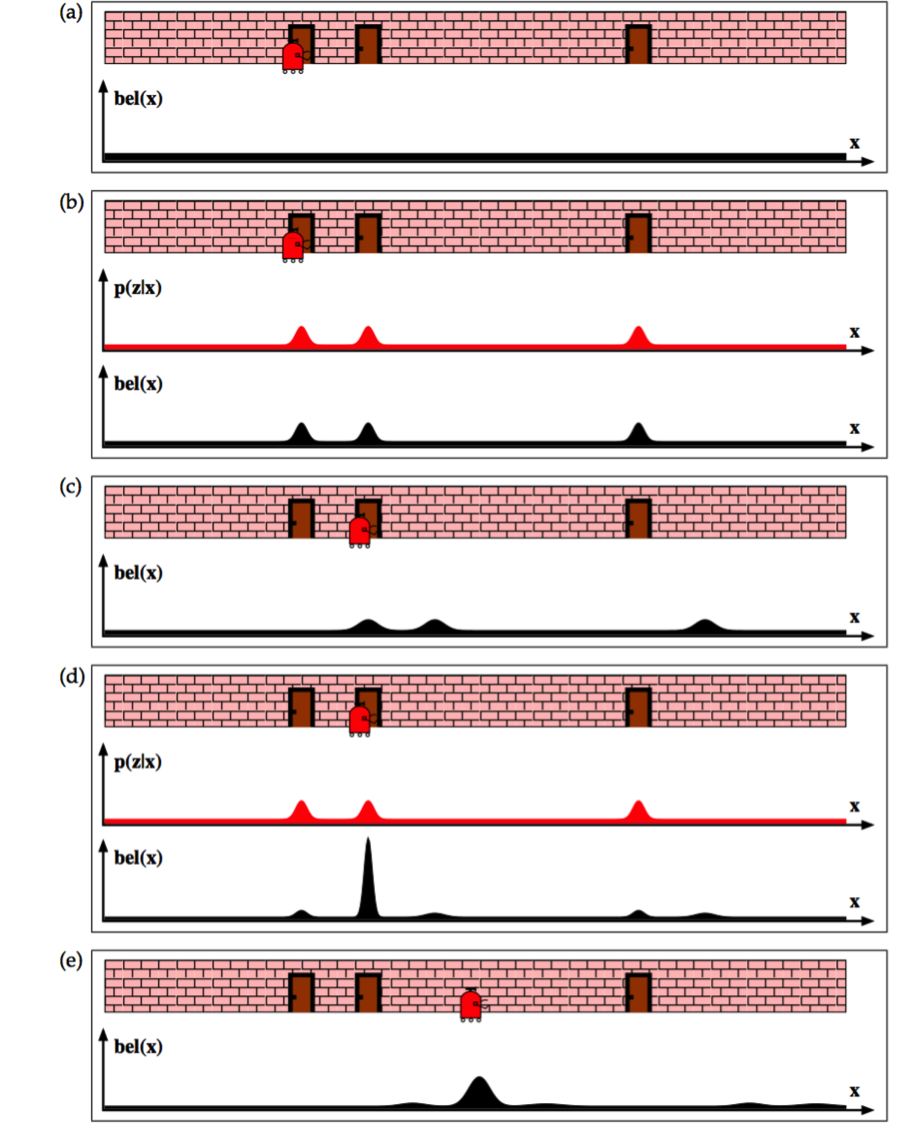
\includegraphics[scale=0.7]{./../img/LocalisationMarkovExemple.png}
\caption{Id�e g�n�rale de la localisation de Markov}
\source{Probabilistic Robotics\cite{Thrun:2005:PR:1121596}}
\end{center}

\label{ILM}
\end{figure}

Les algorithmes probabilistes souffrent de deux d�fauts importants en comparaison aux techniques traditionnelles de programmation en robotique. La premi�re est la complexit� en temps de calcul de l'algorithme qui augmente. En effet, dans les algorithmes probabilistes on consid�re toute la fonction de densit� de probabilit� lorsque les algorithmes classiques ne consid�rent qu'un �l�ment.  La deuxi�me est le besoin d'utiliser des approximations de la densit� de probabilit� exacte. Consid�rer la fonction de densit� exacte devient vite impossible � calculer et est donc indispensable d'utiliser des approximations comme des Gausiennes ou un nombre restreint des �l�ments de la fonction de densit�. Dans certaines situations, ces repr�sentations peuvent �tre �loign�es de la r�alit�. Cependant, l'augmentation de la puissance de calcul des processeurs ainsi que les recherches d'algorithmes plus efficients permettent de grandes �volutions dans le domaine. Toutefois, ces deux points restent encore probl�matiques. Ces deux points sont donc discut�s dans la pr�sentation des algorithmes de localisation suivants.   


\section{Algorithmes de r�solution du probl�me de localisation}
L'algorithme de Markov permet de donner l'id�e g�n�rale des algorithmes de localisation. Cependant pour pouvoir impl�menter concr�tement un algorithme de localisation un certain nombre de questions sont encore ouvertes. La plus importante correspond � la repr�sentation de la fonction de probabilit�. Deux grandes approches existent. La premi�re d�finit une fonction de probabilit� � l'aide de ses param�tres. Et la seconde repr�sente la probabilit� � l'aide d'un certain nombre d'�l�ments discrets. Les sections suivantes discutent de ces deux approches. Elles pr�sentent les algorithmes EKF et MCL qui font partie des algorithmes de localisation les plus connus et qui pr�sentent de bons r�sultats en pratique. 

\subsection{ Algorithme param�trique(EKF)}
Les algorithmes param�triques permettent de repr�senter les croyances de la position d'un robot � l'aide de lois de probabilit�. Les concepts math�matiques de l'algorithme de Kalman ont �t� d�velopp�s dans les ann�es 60 \cite{Kalman61newresults}. Dans le cas de l'algorithme Kalman Filter(KF) la loi de probabilit� est une loi normale. Elle d�pend donc de deux param�tres son esp�rance $\mu$ et son �cart type $\sigma $. Cette loi normale est une loi normale multivari�e lorsque le vecteur de position est compos� de plusieurs �l�ments. On d�finit alors la moyenne de cette fonction multivari�e comme suit  $$\mu = x_t =  \begin{pmatrix} x\\y\\ \theta  \end{pmatrix}$$ 


\begin{algorithm}
\caption{ Kalman filter  }\label{alg:kalmanFilter}
\begin{algorithmic}[1]
\Procedure{KalmanFilter}{$ \mu_{t-1}, \Sigma_{t-1}, u_t, z_t  $}  
\State $ \overline{\mu_t} \gets  A_t \mu_{t-1} + B_t u_t$  \Comment{pr�diction}
\State $ \overline{\Sigma_t } \gets A_t + \Sigma_{t-1} A_t^T+ R_t$ \Comment{pr�diction}
\State $ K_t \gets \overline{\Sigma}_t C_t^T (C_t \overline{\Sigma}_t C^T_t + Q_t )^{-1}$ \Comment{Kalman Gain}
\State $ \mu_t \gets  \overline{\mu}_t  + K_t(z_t - C_t \overline{\mu}_t)  $ \Comment{mise � jour}
\State $ \Sigma_t \gets (I - K_tC_t)\overline{\Sigma}_t$ \Comment{mise � jour}
\State \textbf{return} $ \mu_t,\Sigma_t$
\EndProcedure
\end{algorithmic}
\end{algorithm}

\begin{algorithm}
\caption{ Extended Kalman filter  }\label{alg:ExtendedKalmanFilter}
\begin{algorithmic}[1]
\Procedure{ExtendedKalmanFilter }{$ \mu_{t-1}, \Sigma_{t-1}, u_t, z_t  $}  
\State $ \overline{\mu_t} \gets  g(u_t,\mu_{t-1})$  \Comment{pr�diction}
\State $ \overline{\Sigma_t } \gets G_t \Sigma_{t-1} G_t^T+ R_t$ \Comment{pr�diction}
\State $ K_t \gets \overline{\Sigma}_t H_t^T (H_t \overline{\Sigma}_t H^T_t + Q_t )^{-1}$ \Comment{Kalman Gain}
\State $ \mu_t \gets  \overline{\mu}_t  + K_t(z_t - h(\overline{\mu}_t))  $ \Comment{mise � jour}
\State $ \Sigma_t \gets (I - K_tH_t)\overline{\Sigma}_t$ \Comment{mise � jour}
\State \textbf{return} $ \mu_t,\Sigma_t$
\EndProcedure
\end{algorithmic}
\end{algorithm}


L'algorithme Extended Kalman filter(EKF) correspond � la version non linearaire de l'algorithme du filtre de Kalman. Cette variante a �t� d�velopp�e 
quelques ann�es plus tard  par la NASA\cite{Smith1962} pour faire face au fait que la plupart des syst�mes physiques ne sont pas lin�aires. Pour ce faire les fonctions $g$ et $h$ ont �t� introduites. Ces fonctions ne doivent pas obligatoirement �tre lin�aire mais doivent �tre d�rivables. Contrairement ou filtre de Kalman classique o� les fonctions sont obligatoirement lin�aire pour pr�server des fonctions de r�partition gausienne.



\subsection{Algorithme non param�trique(MCL) }
� l'inverse des algorithmes param�triques, les algorithmes non param�triques ne sont pas bas�s sur une loi de probabilit� connue dont l'algorithme arrange les param�tres pour correspondre au mieux � la croyance de la position. Dans les algorithmes non param�triques, la croyance est repr�sent�e par nombre d�termin� de positions suppos�es. Une probabilit� est associ�e � ces positions suppos�es. Plusieurs techniques existent pour repr�senter ses positions suppos�es. 

La premi�re technique consiste � d�couper la carte de l'environnement en une grille o� chaque �l�ment de la grille correspond � une position suppos�e\cite{4621305}. Pour repr�senter l'orientation du robot, il faut multiplier le nombre de cases par le nombre d'angles d'orientation que peut prendre le robot (voir ~\ref{img:gridMap}).Dans cette repr�sentation, seules trois orientations sont possibles. Ces trois orientations correspondent aux trois plans de la repr�sentation. Comme on peut s'en rendre compte, il est tr�s important de d�finir la bonne granularit� de la d�coupe. Une d�coupe trop importante augmente le temps de calcul, alors qu'une grille trop peu d�coup�e rend la localisation trop peu pr�cise. Dans ce type de d�coupe, plus la carte est grande et plus le temps de calcul est important. 

Dans le cas de l'algorithme de Monte Carlo localization (MCL) aussi appel� Particle filter localization \cite{bib:Rekleitis2004}  car il utilise un filtre � particule, une approche diff�rente a �t� choisie. Dans cet algorithme (voir l'algorithme ~\ref{alg:MCL }) la croyance de la position est repr�sent�e par M particules(voir ~\ref{img:MCL}). Chaque particule est consid�r�e comme une hypoth�se sur la position du robot. Plus une r�gion de la carte contient de particules et plus la probabilit� que le robot s'y trouve est grande. Contrairement aux algorithmes bas�s sur la d�coupe de la carte en une grille, MCL n'implique pas un temps de calcul suppl�mentaire lorsque la taille de la carte augmente. Cependant, il est possible de choisir d'augmenter le nombre de particules pour augmenter la pr�cision. 

MCL souffre d'un probl�me important, en particulier quand $M< 50$ et que l'environnement du robot est grand. Il peut arriver que l'ensemble des particules converge vers une position erron�e. Une fois cette convergence atteinte il est difficile d'en sortir. Pour pallier � ce probl�me, � chaque it�ration un certain nombre de particules sont redistribu�es al�atoirement dans la carte. 

\begin{figure}
\begin{center}
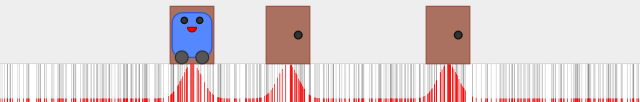
\includegraphics[scale=0.6]{./../img/mcl.png}
\caption{Illustration de MCL, les traits gris correspondent aux particules et le niveau de rouge repr�sente la probabilit� associ�e}
\source{\href{https://en.wikipedia.org/wiki/Monte_Carlo_localization}{Wikipedia}, Auteur : Daniel Lu }
\end{center}

\label{img:MCL}
\end{figure}


\begin{figure}
\begin{center}
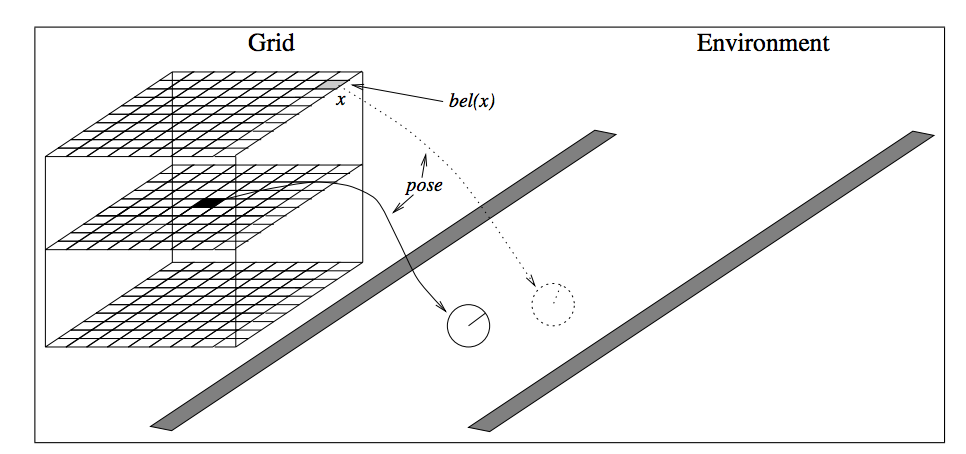
\includegraphics[scale=0.6]{./../img/gridMap.png}
\caption{Illustration de la carte en grille}
\source{Probabilistic Robotics\cite{Thrun:2005:PR:1121596}}
\end{center}
\label{img:gridMap}
\end{figure}



\begin{algorithm}
\caption{ MCL  }\label{alg:MCL }
\begin{algorithmic}[1]
\Procedure{MCL }{$ \mathcal{X}_{t-1}, u_t, z_t ,m $}  
\State $ \overline{\mathcal{X}_t} \gets  \emptyset $  
\State $ \mathcal{X}_t \gets  \emptyset $  

\For {$ m = 1$ to  M }
\State  $ x^{[m]}_t \gets sample\_motion\_model(u_t , x^{[m]}_{t-1})$
\State $w_t^{[m]} \gets measurement\_model(z_t , x_t^{[m]},m)$
\State $ \overline{\mathcal{X}}_t \gets \overline{\mathcal{X}}_t + \langle  x^{[m]}_t , w_t^{[m]} \rangle $
\EndFor

\For {$ m = 1$ to  M }
\State draw i  with probability $\propto w^{[i]}_t$
\State add $x^{[i]}_t$ to $\mathcal{X}_t$
\EndFor
\State \textbf{return} $ \mathcal{X}_t$
\EndProcedure
\end{algorithmic}
\end{algorithm}


\subsection{Comparaison de MCL et EKF}
Le tableau ~\ref{MCLVSEKF} donne et compare les principales caract�ristiques de l'algorithme EKF et MCL. Ce tableau comparatif permet de mettre en valeur qu'aucun algorithme n'est globalement meilleur. Ils poss�dent chacun leurs qualit�s et d�fauts. Les d�fauts de l'un se r�v�lent les qualit�s de l'autre. Par exemple, EKF est efficient en temps et m�moire contrairement au MCL dont l'efficience d�pend fortement du nombre de particules. 

Cependant, MCL est plus robuste � EKF. En effet, la repr�sentation de la fonction de probabilit� � l'aide d'une loi normale permet � EKF d'�tre efficient. Cependant, le revers de cette efficience est qu'il est moins robuste lorsque la fonction de probabilit� est fortement diff�rente d'une loi normale. Prenons l'exemple d'un long couloir avec un grand nombre de portes et o� le robot n'est pas capable de distinguer les portes. Dans cette situation MCL peut donner de meilleures performances. En effet, EKF assume que la croyance de la position est proche d'une distribution gaussienne et a donc de mauvaises performances lorsque la croyance correspond plut�t � distribution multimodale. Pour pallier � ce probl�me, l'algorithme classique EKF a �t� am�lior�. Multi-hypothesis tracking (MHT)\cite{1263228} filtre permet de repr�senter la croyance � l'aide d'un mixte de plusieurs gaussienne et donc d'avoir un algorithme plus robuste et efficient.

La localisation globale correspond � un probl�me de localisation o� la position initiale n'est pas connue et l'incertitude est donc grande � cet instant. Il s'av�re qu' EKF est plus appropri� pour suivre la position d'un robot dont on connait d�j� la position initiale. En effet, une repr�sentation unimodale est g�n�ralement une bonne repr�sentation dans un probl�me o� il s'agit de suivre une position, mais pas dans un probl�me de localisation globale. La lin�arisation dans EKF ne fait qu'accroitre ce probl�me en risquant de converger vers une mauvaise position.


De plus, MCL permet de traiter directement dans l'algorithme des mesures brutes or EKF n�cessite des rep�res. Il est donc possible � l'aide de MCL d'utiliser directement les valeurs de capteurs de distance entre le robot et des murs pour les comparer avec une carte repr�sentant les murs. Ce qui n'est pas possible � l'aide de EKF qui n�cessite une carte compos�e d'un nombre limit� de rep�res qui permet de localiser le robot � l'aide des rep�res mesur�s dans son environnement. Finalement, en pratique il s'av�re que MCL est plus simple � impl�menter qu'EKF.


\begin{table}
\begin{center} 

\begin{tabular}{l | c | c }
               & EKF & MCL \\
               \hline
Mesures & Rep�res & Brute \\ 
Erreur de Mesure & Gaussienne & Toute \\
Posterior &Gaussienne & Particules \\
Efficience(m�moire) & ++ & + \\
Efficience(temps)& ++ & + \\
Facilit� d'impl�mentation & + & ++ \\
R�solution & ++ & + \\
Robuste & - & ++ \\ 
Localisation Globale & non & oui\\ 
\hline 
\end{tabular}
\caption{Comparaison EKF et MCL}
\label{MCLVSEKF} 
\end{center}
\end{table}


\section{Simultaneous Localization And Mapping}
Les algorithmes Slam (Simultaneous Localization And Mapping) sont l'�tape suivante de l'ind�pendance des robots. En effet, dans les algorithmes de simple localisation, la carte de l'environnement doit �tre construite avant de la passer en param�tre aux algorithmes de localisation. Comme son nom l'indique, dans un algorithme Slam la carte est construite en parall�le avec la localisation du robot. 

\begin{algorithm}
\caption{ EKFSLAM  }\label{alg:EKFSLAM }
\begin{algorithmic}[1]
\Procedure{EKFSLAM }{$ \mu_{t-1}, \Sigma_{t-1},  u_t , z_t, m,c_t  $}  
\State $ F_x \gets 
\begin{pmatrix}
1&0& 0\\
0&1&0\\
0&0&1\\
\end{pmatrix}
$


\State $\overline{\mu}_t \gets \mu_{t-1} +  F^T_x
\begin{pmatrix}
d \cos \\
d \sin \\
\gamma \\
\end{pmatrix}
$

\State $G_t \gets I + F_x^T 
\begin{pmatrix}
0,0\\
0,0\\
0,0\\
\end{pmatrix}$


\State $\overline{\Sigma}_t \gets G_t \Sigma_{t-1}G_t^T + F_x^TR_tF_x $

\State $ Q_t \gets 
\begin{pmatrix}
\sigma^2_r&0&0\\
0&\sigma^2_r&0\\
0&0&\sigma^2_r\\
\end{pmatrix}$

\ForAll{ observed features   {$ z^i_t \gets (d^i_t,\rho^i_t)^T $ }}
\State $j \gets c_t^i$
\If{landmark j never seen before}
\State $
\begin{pmatrix}
\overline{\mu}_{j,x}\\
\overline{\mu}_{j,y}\\
\end{pmatrix}
\gets 
$ 
\EndIf
 
\State $q \gets (m_{j,x}-\overline{\mu}_{t,x} )^2 + (m_{j,y}-\overline{\mu}_{t,y})^2$
\State $ \hat{z}^i_t \gets 
\begin{pmatrix}
\sqrt{q}\\
atan2(m_{j,y}-\overline{\mu}_{t,y},m_{j,x}-\overline{\mu}_{t,x} )- \overline{\mu_{t,\theta}}\\
\end{pmatrix}
$
\State $H^i_t \gets
\begin{pmatrix}
-\frac{m_{j,x}-\overline{\mu}_{t,x}}{\sqrt{q}}     &    -\frac{m_{j,y}-\overline{\mu}_{t,y}}{\sqrt{q}}   &    0\\
\frac{m_{j,y}-\overline{\mu}_{t,y}}{q} & -\frac{m_{j,x}-\overline{\mu}_{t,x}}{q}            &  -1\\

\end{pmatrix}
$ 

\State $S^i_t \gets H^i_t \overline{\Sigma_t} [H^i_t]^T + Q_t $ 
\State $ K_t^i \gets \overline{\Sigma}_t [H_t^i]^T [S^i_t ]^{-1}$ \Comment{Kalman Gain}

\State $ \overline{\mu}_t \gets  \overline{\mu}_t  + K_t^i(z_t^i - \hat{z}^i_t ))  $ \Comment{mise � jour}
\State $ \overline{\Sigma}_t \gets (I - K_t^iH_t^i)\overline{\Sigma}_t$ \Comment{mise � jour}

\EndFor

\State $ \mu_t \gets  \overline{\mu}_t $  

\State $ \Sigma_t \gets \overline{\Sigma}_t $  

\State \textbf{return} $ \mu_t , \Sigma_t $
\EndProcedure
\end{algorithmic}
\end{algorithm}


\part{Impl�mentations }
Cette partie d�crit l'impl�mentation de l'algorithme EKF sur la brique EV3. Il y est �galement pr�sent� un algorithme qui utilise la position du robot pour construire une grille d'occupation.  Cette grille d'occupation sert � construire un graphe qui permet de trouver un chemin entre un point de d�part et un point d'arriv�e de la carte. En plus de ces descriptions d'algorithmes, cette partie aide le lecteur qui souhaite d�velopper un algorithme sur son propre robot. Une description de la brique EV3, de ses capteurs et des possibilit�s de programmation qu'offre la brique EV3 est donn�e pour aider ce lecteur dans cette aventure. De plus, des conseils sur la construction du robot sont �galement donn�s pour permettre au d�veloppeur de construire un bon ch�ssis pour son robot. Finalement, des alternatives � la brique EV3 sont donn�es. En effet, cette brique est relativement couteuse et elle ne r�pond pas toujours au besoin du d�veloppeur. C'est pourquoi cette partie contient une pr�sentation de quelques simulateurs en robotique ainsi que la pr�sentation des microcontr�leurs Arduino et Raspberry Pi.   


\chapter{Lego Mindstorms}
Les Legos sont des jouets de construction fabriqu�s par le groupe danois �~The Lego Group�. La s�rie Mindstorms correspond � la gamme �~robotique programmable~� de Legos. Cette s�rie est vendue en kits qui permettent de r�aliser certains mod�les de robots pr�d�finis et par la suite de laisser cours � son imagination. Les kits contiennent une brique intelligente programmable, un ensemble de capteurs et de moteurs ainsi qu'un ensemble d'�l�ments de construction qui proviennent de la gamme Lego Technic. Ces kits permettent de r�aliser rapidement et � couts mod�r�s des robots simples. Ils se sont donc vite r�v�l�s comme des outils int�ressants pour l'apprentissage de la robotique et de la programmation.

\section{Description du hardware}
Le kit Lego peut �tre compar� � des packs compos�s de microcontr�leurs Arduino\footnote{Arduino : \href{https://www.arduino.cc}{www.arduino.cc} } ou Raspberry Pi\footnote{Raspberry Pi : \href{https://www.raspberrypi.org}{www.raspberrypi.org}  } et d'une s�rie de capteurs et de moteurs. Les microcontr�leurs Arduino et Raspberry Pi poss�dent l'avantage de pouvoir utiliser une plus grande gamme des capteurs et moteurs � moindres couts. Cependant, la mise en place de ces capteurs se r�v�le de plus bas niveau et donc plus longue. Contrairement au kit Lego o� les moteurs et capteurs sont de type �plug and play�. Ce projet est plus bas� sur les aspects de programmation en robotique que sur les aspects hardware, c'est pourquoi le kit Lego Mindstorms a �t� favoris�. 


\subsection{Brique intelligente}
La brique intelligente programmable (voir Figure ~\ref{EV3} ) est le cerveau des robots EV3. Elle est dot�e d'une interface � six boutons lumineux qui changent de couleur pour indiquer l'�tat d'activit� de la brique, d'un affichage � haute r�solution noir et blanc, d'un hautparleur int�gr�, d'un port USB, d'un lecteur de cartes mini SD, de quatre ports d'entr�e et de quatre ports de sortie. La brique prend �galement en charge la communication USB, Bluetooth et Wifi avec un ordinateur. Son interface programmable permet � la fois de programmer et de journaliser des donn�es directement sur la brique. Elle est compatible avec les appareils mobiles et est aliment�e par des piles AA ou par la batterie CC rechargeable EV3. La brique EV3 fournit l'�nergie pour les capteurs et les moteurs. Elle permet de r�cup�rer et de traiter les informations des capteurs et d'envoyer des commandes aux moteurs par l'interm�diaire des ports d'entr�e et de sortie. Ce qui rend la connexion et l'utilisation des capteurs et des moteurs tr�s facile.

\begin{figure}
\begin{center}
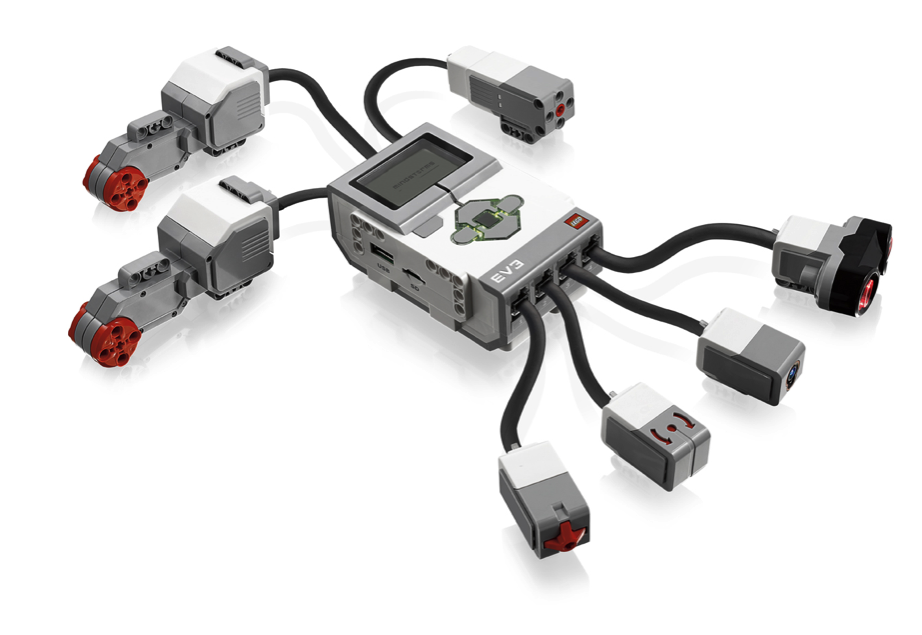
\includegraphics[scale = 0.7]{./../img/EV3.png}
\caption{Brique EV3}
\source{ \href{http://www.4erevolution.com/lego-mindstorm-ev3-hacking/}{www.4erevolution.com}}
\end{center}

\label{EV3}
\end{figure}


Depuis son lancement la gamme de Lego Mindstorms a connu trois types de briques qui se sont succ�d�s, la brique RXC, NXT et EV3. Elles ont progressivement augment� de puissance de calcul. La vraie r�volution de la brique EV3 est la possibilit� de booter le syst�me sur une carte SD. Ce qui augmente ainsi le potentiel de la brique (comme d�crit dans la section ~\ref{sec:DesSoftware}). 

La brique EV3 embarque un processeur arm9, 16Mo de m�moire flash et 64Mo de RAM. La carte SD permet d'�tendre la m�moire � 32Go. Il est vrai que la puissance a augment� dans la brique EV3 en comparaison avec ses pr�d�cesseurs. Toutefois, cette puissance de calcul reste r�duite en comparaison aux ordinateurs et smartphones actuels. 
\subsection{Moteurs et capteurs}
Le pack de base de la brique EV3 est compos� de deux moteurs moyens, un petit moteur, un capteur de pression, un capteur de distance infrarouge et d'un capteur de couleurs. Il est possible d'acheter des capteurs Legos suppl�mentaires tels qu'un gyroscope, un capteur de distance ultrasonique et une boussole. Il est �galement possible d'acheter d'autres types de capteurs d�velopp�s par des soci�t�s ind�pendantes de Lego. C'est possible gr�ce au support de protocoles standards que doivent adopter les capteurs de donn�es. On peut par exemple citer $I^2C$ qui est un bus de donn�es con�u par Philips et qui est tr�s r�pandu dans le monde de l'�lectronique. On voit donc en vente des capteurs GPS, des capteurs RFID, des capteurs d'humidit� qui sont compatibles avec la brique EV3

La partie qui suit d�crit plus en profondeur les capteurs et moteurs du kit de base qui sont ceux disponibles pour r�aliser ce projet. Les descriptions sont bas�es sur les informations donn�es par le constructeur. Les descriptions sont dirig�es vers le type de donn�es re�ues ainsi que la pr�cision des capteurs et des moteurs. Ces descriptions sont importantes dans ce m�moire, car elles permettent de mieux connaitre les capteurs et les moteurs � notre disposition ce qui permet ainsi de mieux d�finir les erreurs qui sont propres � ces capteurs.

Le capteur infrarouge EV3 d�tecte la proximit� d'objets (jusqu'� 70 cm) et lit les signaux �mis par la balise infrarouge EV3 (distance max de 2m ). Les utilisateurs peuvent cr�er des robots t�l�command�s, faire des courses d'obstacles et se familiariser avec l'utilisation de la technologie infrarouge. Cette technologie est pr�sente dans les t�l�commandes des TV, les syst�mes de surveillance.

Le capteur de couleur num�rique EV3 diff�rencie huit couleurs. Il peut �tre utilis� aussi comme capteur photosensible en mesurant l'intensit� lumineuse. Les utilisateurs peuvent construire des robots qui trient selon les couleurs ou suivent une ligne, exp�rimenter la r�flexion de la lumi�re de diff�rentes couleurs et se familiariser avec une technologie largement r�pandue dans les secteurs industriels du recyclage, de l'agriculture et de l'emballage. 

Le capteur tactile analogique EV3 est un outil simple, mais extr�mement pr�cis, capable de d�tecter tous les pressions ou les rel�chements de son bouton frontal. Les utilisateurs pourront construire des syst�mes de commande marche/arr�t, cr�er des robots capables de s'extraire d'un labyrinthe et d�couvrir l'utilisation de cette technologie dans des appareils tels que les instruments de musique num�riques, les claviers d'ordinateur ou l'�lectrom�nager.

Le grand servomoteur EV3 est un puissant moteur avec retour tachym�trique pour un contr�le pr�cis au degr� pr�s. Gr�ce � son capteur de rotation int�gr�, ce moteur intelligent peut �tre synchronis� avec les autres moteurs d'un robot pour rouler en ligne droite � la m�me vitesse. Il peut �galement �tre utilis� pour fournir une mesure pr�cise pour des exp�riences. Par ailleurs, la forme du boitier facilite l'assemblage des trains d'engrenage.

Le servomoteur moyen EV3 est parfait pour des charges moins importantes, des applications � vitesse plus �lev�e, ainsi que des situations o� une plus grande r�activit� et un plus petit profil sont n�cessaires lors de la conception du robot. Le moteur se sert d'un retour tachym�trique pour un contr�le pr�cis au degr� pr�s et il poss�de un capteur de rotation int�gr�.

\subsection{Simulateurs}
 Pour les personnes qui ne souhaitent pas acheter de mat�riels ou pour des tests � plus grande �chelle, il est possible d'utiliser des simulateurs. Un simulateur comme Gazebo \footnote{Gazebo : \href{http://gazebosim.org/}{gazebosim.org}} permet d'utiliser ou de construire des mod�les de robots qui �voluent dans un environnement pr�d�fini. Ce projet open source  a re�u des financements de la DRC\footnote{DRC : \href{http://www.theroboticschallenge.org/}{www.theroboticschallenge.org}} pour l'adaptation du simulateur � son robot ATLAS. Cependant, ce type de simulateur n�cessite un temps d'apprentissage certain pour pouvoir commencer � l'utiliser. C'est pourquoi d'autres simulateurs plus simples de la brique de Lego existent. L'universit� de Berne a d�velopp� EV3JLIB\footnote{EV3JLIB : \href{http://www.aplu.ch/home/apluhomex.jsp?site=145}{www.aplu.ch}} qui permet de lancer gratuitement un simulateur en ligne. Le comportement du robot est cod� en Java. Ce code a l'avantage d'�tre r�utilisable sur la brique. D'autres logiciels destin�s � l'apprentissage de la robotique � l'aide d'un simulateur de la brique EV3 et plus �volu�s graphiquement que EV3JLIB sont disponibles en ligne. Les deux principaux sont �virtual robotics toolkit� \footnote{Virtual robotics toolkit :  \href{https://cogmation.com/virtual-robotics-toolkit}{cogmation.com} }et   �Robot virtual worlds� \footnote{Robot virtual worlds : \href{http://www.robotvirtualworlds.com/virtualbrick/}{www.robotvirtualworlds.com}} mais ils sont payants.

\section{Description du software } 
\subsection{RoboLab}
\label{sec:DesSoftware}
C'est dans la brique EV3 qu'il est possible d'injecter un programme contenant les instructions du robot. Lego fournit un langage de programmation graphique qui s'appelle RoboLab(voir ~\ref{Robolab}). Ce langage de programmation est constitu� d'un ensemble de briques. Il est possible de les assembler pour d�finir le mini programme qui d�finit le comportement du robot. Les briques permettent de d�finir des actions sur les moteurs, afficher des messages sur l'�cran de la brique EV3, jouer des sons. Il est �galement possible de d�finir des conditions � l'aide des valeurs obtenues par les capteurs et m�me de lancer des boucles. Il est le fruit de la collaboration de Lego avec le M.I.T.. Il se r�v�le un bon langage de programmation pour l'apprentissage de la programmation. Cependant, il n'est pas appropri� au d�veloppement d'algorithmes complexes de localisation comme EKF ou bien MCL. Les briques Mindstorm ont vite �t� hack�es pour permettre de d�velopper des programmes � l'aide d'autres langages que RoboLab. Dans la version EV3, il est possible de booter sur une carte SD. Ce qui a permis que des OS tels que Linux soient adapt�s pour fonctionner sur la brique. Le projet ev3Dev est un exemple d'adaptation de Linux pour la brique EV3. Il est donc maintenant potentiellement possible de d�velopper � l'aide de tous les langages disponibles sur Linux. Lejos est une API �crite en Java comme le laisse supposer son nom. Lejos est l'outil principalement utilis� dans ce m�moire, une description plus compl�te est donc donn�e dans une section d�di�e.

\begin{figure}
\begin{center}
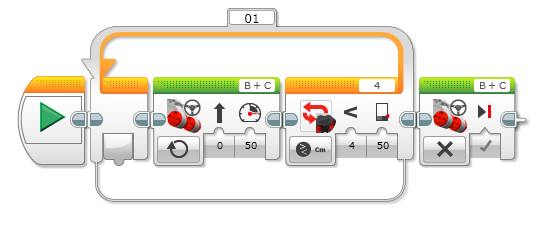
\includegraphics[scale=0.7]{./../img/Robolab.png}
\caption{Robolab}
\source{\href{http://www.lego.com/en-us/mindstorms/}{www.lego.com}}
\end{center}
\label{Robolab}
\end{figure}



\subsection{Lejos}
Lejos est un microprogramme libre destin� � remplacer le microprogramme originalement install� sur la brique Lego Mindstorm. Il est disponible sur les briques RCX, NXT et EV3. Lejos inclut une machine virtuelle Java permettant de d�velopper des robots dans le langage Java. Ce qui a donn� le nom Lejos qui est le mot Legos o� le � g � a �t� remplac� par un � j � pour Java. Pour la version EV3 de la brique Lego, cette machine virtuelle Java est mise � disposition par Oracle. Lejos permet un acc�s facile aux moteurs et aux capteurs. Ce qui est possible gr�ce aux routines �crites en c et mise dans le domaine public par le groupe Lego. En effet, Lego � d�cider de publier le code source de la brique EV3 en open source. Ces routines en c permettent en th�orie d'utiliser n'importe quel langage de programmation pour d�velopper des comportements de robots. 

Depuis son lancement jusqu'� aujourd'hui Lejos dispose d'une communaut� active et de taille assez importante. Le d�p�t officiel du code source est sourceforge.net. Entre le 01-01-2015 et le 09-04-2015 la version 0.9.0-beta de la brique EV3 a �t� t�l�charg�e 2700 fois. En effet, l'outil Lejos est couramment utilis� dans les universit�s et dans les hautes �coles pour l'apprentissage de la robotique et du langage Java. L'impl�mentation orient�e objet permet aux �tudiants d'�tudier la robotique avec le niveau d'abstraction qu'ils d�sirent. Il est ainsi possible de d�velopper des algorithmes de localisation sans se soucier des adresses hexad�cimales des moteurs et des capteurs. 

Lejos est �galement utilis� dans la recherche. De nombreux projets ont d�j� vu le jour. Des chercheurs de l'universit� de Porto au Portugal ont d�j� utilis� Lejos pour impl�menter un algorithme  qui cartographie l'environnement d'un robot \cite{OliveiraLejos}. Encore � l'universit� de Porto un simulateur simple et des exercices d'utilisation de l'algorithme EKF ont �t� d�velopp�s\footnote{ EKF : \href{http://paginas.fe.up.pt/~robosoc/en/doku.php?id=start_lego}{paginas.fe.up.pt/~robosoc}} par les professeurs de l'universit� de Porto. Un �tudiant su�dois a d�velopp� un SLAM\footnote{ SLAM : \href{http://penemunxt.blogspot.be/}{penemunxt.blogspot.be}} et des outils de visualisation de la carte et de la position du robot. Finalement, un projet qui permet de d�finir le comportement d'un robot � l'aide de diagramme d'�tat est disponible sur github\footnote{ Diagramme d'�tats : \href{https://github.com/jabrena/liverobots}{github.com/jabrena/liverobots}}. L'ensemble de ces projets prouve que Lejos poss�de de bonnes bases pour d�velopper des algorithmes complexes. 

\section{Description du robot construit}
La plateforme du robot construit est de type �~differential wheeled robot~�(voir ~\ref{DWR}). Ce qui consiste en deux moteurs ind�pendants positionn�s de fa�on oppos�e sur le robot. En plus de ses deux roues, une roue libre est plac�e � l'arri�re. Il est conseill� de ne pas placer cette roue libre au centre de l'axe de rotation vertical de celle-ci pour cr�er un levier qui garantit une meilleure rotation de cette roue libre. Ce choix de plateforme est commun en robotique. Cette plateforme est simple � mettre en oeuvre et fournit une amplitude de mouvement importante. A l'inverse les plateformes de type steering sont semblables aux voitures classiques. Elles demandent un m�canisme plus complexe et leur amplitude de mouvement est moindre et donc moins adapt�e � la robotique.

\begin{figure}
\begin{center}
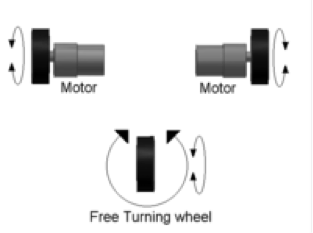
\includegraphics{./../img/DifferentialWheeledRobot.png}
\caption{Differential wheeled robot }
\source{\href{https://en.wikipedia.org/wiki/Differential_wheeled_robot}{Wikipedia},
 Auteur : Patrik}
 \label{DWR}
\end{center}

\end{figure}

La figure ~\ref{Robot} pr�sente le robot qui a �t� construit pour r�aliser l'impl�mentation et tester les algorithmes pr�sent�s dans ce m�moire. Le robot est compos� d'un capteur de pression. Il n'est pas possible de d�terminer la localisation d'une pression sur le pare-chocs avant. La pression est identifi�e indiff�remment que ce soit le c�t� gauche ou le c�t� droit du pare-chocs qui a �t� touch�. Il est �galement �quip� d'un capteur de distance infrarouge sur sa face avant. Un support est plac� sur le haut du robot pour accueillir le smartphone qui s'occupe de scanner les codes QR qui sont les points de rep�re du robot dans l'algorithme EKF. Pour permettre � la brique EV3 de communiquer de fa�on efficace avec le smartphone et l'ordinateur un stick USB wifi a �t� ajout� � la brique EV3. La communication avec l'ordinateur doit �tre efficace pour permettre que les donn�es capt�es par les capteurs de la brique EV3 soient rapidement envoy�es � l'ordinateur et inversement pour que les commandes envoy�es par l'ordinateur arrivent rapidement sur la brique EV3.

La construction de la plateforme de d�placement et l'ajout des capteurs sur le robot sont des �tapes � ne pas n�gliger. Elle est relativement longue pour avoir un robot utilisable. En effet, il est important de positionner les capteurs et les moteurs � des endroits r�fl�chis. Il est par exemple primordial de ne pas placer des �l�ments de la plateforme devant le capteur de distance. Le pare-chocs muni du capteur de pression doit �tre construit de fa�on � bien r�agir � tous les types de chocs. L'ensemble des c�bles doit �tre introduit dans les ports appropri�s de la brique EV3 sans entraver le fonctionnement des moteurs ou des capteurs. Finalement, certaines propri�t�s du robot permettent de simplifier leur manipulation et les algorithmes qui sont impl�ment�s pour les manipuler. Il est par exemple plus simple de manipuler un robot avec un ch�ssis arrondi et capable de faire un demi-tour sur lui-m�me. Il est possible � l'aide d'un ch�ssis arrondi de faire facilement un demi-tour sur soi-m�me dans un angle d'un mur sans le percuter. Alors qu'un ch�ssis de type rectangulaire a tendance � se bloquer l'or de la rotation pour faire le demi-tour. En effet, les coins du robot ont tendance � percuter le mur. Dans le cas d'un robot rectangulaire, les algorithmes de mouvement doivent prendre en compte les particularit�s de la forme du robot pour �viter de percuter des objets. L'ensemble des contraintes de construction des robots rend compliqu�e la construction d'un robot. Il est donc possible de trouver sur le web des exemples de plateformes qui ont fait leurs preuves. Le site nxtprograms \footnote{ nxtprograms : \href{http://www.nxtprograms.com/index2.html}{www.nxtprograms.com}} propose une s�rie d'exemples de plateformes �volutives.  



\begin{figure}
\begin{center}
\includegraphics[scale=0.7]{./../img/EV3Robot.png}
\caption{Robot }
\label{Robot}
\end{center}
\end{figure}



 

\chapter{Algorithme de localisation}
Cette section contient la description de l'impl�mentation de l'algorithme EKF r�alis�e pour ce m�moire. Par la suite, l'impl�mentation de l'algorithme EKF est compar�e � l'impl�mentation MCL d�j� pr�sente dans la librairie Lejos. 




\section{Algorithme EKF }

\subsection{Odom�trie}
L'odom�trie permet de determiner les mouvements $u_t$ n�cessaire � l'�tape de pr�diction de chaque it�ration de l'algorithme EKF. Pour d�terminer le mouvement $u_t$ l'odom�trie consiste � compter le nombre de rotation des moteurs et d'y associer le mouvement correspondant en fonction du chassis du robot. Il est n�cessaire de connaitre la taille des roues ainsi que leur �cartement pour d�terminer le mouvement en fonction du nombre de tour des moteurs. Dans le cas d'un robot �Differential wheeled� les formules sont les  suivantes : 
$$
d =   \frac{d_1 + d_2}{2}
$$
$$
\rho =\frac{d_1-d_2}{b}
$$

o� $d_1 $ et $d_2$ correspondent respectiment � la distance parcourue par les roues 1 et 2. Et $b$ correspond � l'�cart entre les deux roues. $d_1$ et $d_2$ est calcul� en multipliant le nombre de tour des capteurs multiplier par la circonf�rence de la roue  
$$d_1 = 2*\pi R_1$$ 
o� $R1$ est le rayon de la roue 1. Les mouvements doivent �tre soit une ligne droite soit une rotation pour pouvoir appliquer le mod�le de mouvement qui rappelons le est compos� d'une premi�re rotation suivi d'un mouvement en ligne droite. Cette repr�sentation n'est pas restrictive. En effet, il est possible de d�couper la trajectoire en un ensemble de sous mouvement compos� de ligne droit et de rotation.  

\subsection{D�tection de rep�res}
\label{sec:Detection de Feature avec la camera du smartphone}

Les codes QR sont des �l�ments faciles � identifier pour la cam�ra d'un smartphone. De nombreuses librairies de qualit� ont d�j� �t� d�velopp�es pour d�tecter et d�coder des codes QR. Zbar \footnote{ Zbar : \href{http://zbar.sourceforge.net/}{zbar.sourceforge.net}} est une de ces librairies open source. Elle est disponible sur Android et  IOS.  Pour ce m�moire, une application permettant d'estimer la distance du smarphone au code QR a �t� d�velopp�e � l'aide de la librairie Zbar. Pour pouvoir utiliser les codes QR pour estimer la distance entre eux et le smartphone, les codes QR doivent �tre d'une dimension donn�e (dans ce m�moire : un carr� de 10cm de cot� ). La librairie Zbar renvoie la dimension du code QR en nombre de pixels capt�s par la cam�ra. � l'aide d'un �talonnage de la cam�ra qui consiste � d�terminer l'ouverture de l'objectif et du calcul trigonom�trique suivant, il est possible de d�terminer la distance des codes QR de 10cm de cot�(voir ~\ref{EDQRC}).
$$Distance =  \frac{\frac{CapteurResolutionHorizontale }{MesureNombrePixelsHorizontale} * LargeurCodeQR}  {2*\tan(\alpha)} $$


\begin{figure}
\begin{center}
\begin{tikzpicture}

    % define coordinates
    \coordinate (O) at (0,0) ;
    \coordinate (A) at (6,0) ;
    \coordinate (B) at (-2,0) ;

    \coordinate (E) at (3,3) ;
    \coordinate (F) at (3,-3) ;
    
   \coordinate (A_QR_R) at (3,1) ;
   \coordinate (B_QR_R) at (3,2) ;
   \coordinate (M_QR_R) at (3,1.5) ;
   
   



    % axis
    \draw[] (A) -- (B) ;
    

      \draw[blue] (E) -- (F) ;
      \draw[red,ultra thick] (A_QR_R) -- (B_QR_R) ;
      \node[right,red] at (3,1){Code QR de 10cm};
        \node[right,blue] at (3,-1){Vue globale du smartphone};
      
      \fill[black] (M_QR_R) circle (2pt);
      \draw[dash pattern=on5pt off3pt,ultra thick] (O) -- (M_QR_R) ;



    % rays
    \draw[dash pattern=on5pt off3pt,red,ultra thick] (O) -- (45:5);
    \draw[dash pattern=on5pt off3pt,red,ultra thick] (O) -- (-45:5);

    % angles
    \draw[ultra thick,red] (0.7,0) arc (0:45:0.7);
        \draw[ultra thick,black] (1.5,0) arc (0:26:1.5);
    \node[black] at (10:1.9)  {$\theta$};

    \node[red] at (10:0.9)  {$\alpha$};
    
    
\end{tikzpicture}
\end{center}
\caption{�valuation de la distance des codes QR}
\label{EDQRC}
\end{figure}

Il est �galement possible de d�terminer l'angle entre la direction du robot et le centre du code QR � l'aide de la formule suivante : 

$$\theta = \alpha-\frac{\alpha * 2*CentreCodeQRPixel}{ CapteurResolutionHorizontale} $$
si le code QR se trouve � droite du robot la formule devient :
$$\theta = \frac{\alpha * 2*CentreCodeQRPixel}{ CapteurResolutionHorizontale}-\alpha $$

L'�talonnage consiste � d�terminer $\alpha $ � l'aide de mesures faites � distance connue. 




\subsection{Les cartes }
La carte qui stocke les positions des codes QR  et qui est utilis�e par l'algorithme EKF est stock�e dans une image au format SVG. Ce format consiste � d�finir des �l�ments graphiques simples dans un fichier XML. Les codes QR sont donc repr�sent�s par une ligne de 10cm de longueur. La figure ~\ref{ekfmap} repr�sente cette carte o� les codes QR sont repr�sent�s en rouge et les murs en noir. 
Les murs sont �galement d�finis dans un fichier SVG diff�rent. Cette d�composition des cartes est volontaire et elle permet de charger uniquement les sous-cartes utiles � l'algorithme. Il n'est par exemple pas utile pour l'algorithme MCL d'avoir la carte compos�e des codes QR.  

En plus, de ces deux cartes qui ont �t� g�n�r�es � la main au pr�alable. Une carte dynamique de type grille d'occupation est g�n�r�e � l'aide du capteur infrarouge et du capteur de pression positionn�e � l'avant du robot. 


\begin{figure}
\begin{center}

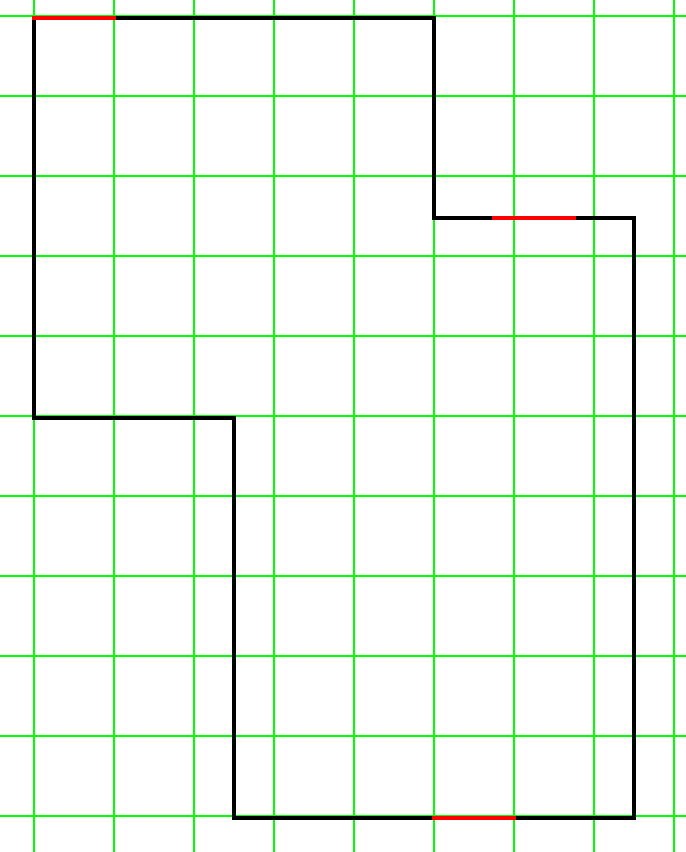
\includegraphics[scale=0.6]{./../img/ekfmap.png}
\caption{carte EKF }
\label{ekfmap}
\end{center}
\end{figure}  

\subsection{Pseudo-code}

L'impl�mentation EKF utilise la technique de d�tection de codes QR comme features pr�sent�es dans la section ~\ref{sec:Detection de Feature avec la camera du smartphone}. 


Cette impl�mentation d'EKF compl�te la librairie Commons Math\footnote{Commons Math : \href{http://commons.apache.org/proper/commons-math/}{commons.apache.org/proper/commons-math}}  qui est une librairie math�matique open-source de Apache. Celle-ci contient une s�rie de classe permettant de manipuler et d'appliquer des op�rations sur des matrices. Ce qui se r�v�le tr�s utile dans les algorithmes de Kalman. Elle contient �galement une impl�mentation du filtre de Kalman, mais ne contient pas d'impl�mentation du Extended Kalman Filter. 

\subsection{Matrice de covariance}
\label{sectionCovariance}
La matrice de covariance est comme son nom l'indique une matrice qui permet de repr�senter la covariance entre chaque variable de la position du robot. Les valeurs contenues dans cette matrice sont tr�s utiles, mais restent fastidieuses � lire, car cette matrice change dynamiquement et r�guli�rement. Il a donc �t� important d'impl�menter une repr�sentation graphique des informations importantes de cette matrice de covariance. Cette repr�sentation permet de se faire une id�e rapide de ces valeurs, sans devoir les analyser une � une. La figure~\ref{cov} pr�sente la repr�sentation choisie de la covariance. La moyenne donne la position estim�e du robot. Cette position estim�e est repr�sent�e par le point bleu central qui correspond � la position $x,y$ estim�e du robot et la droite bleue au milieu des deux autres correspond � la direction estim�e du robot. L'ellipse autour de la position ainsi que les deux autres droites permettent de repr�senter la matrice de covariance. Voici la d�finition de la covariance pour mieux comprendre ce que repr�sente la covariance et comprendre comment sont construites cette ellipse et ces droites  : 

$$ Cov(X,Y) = E[(X-E[X])(Y-E[Y])]  $$  
o� $E[] $ d�signe l'esp�rance math�matique. La covariance caract�rise la variation simultan�e des deux variables al�atoires $X, Y$. Elle est positive lorsque la diff�rence entre les variables al�atoire $X,Y$ et leur moyenne ont tendance � �tre de m�me signe et n�gative dans le cas contraire. Soit le vecteur de position �crit :
$$\vec{X} = \begin{pmatrix} x \\ y \\ \theta \\ \end{pmatrix}$$

La matrice de covariance pour le vecteur de position est la suivante :

$$Var(\vec{X})= 
\begin{pmatrix} 
Var(x) & Cov(x,y)& Cov(x,\theta) \\ 
Cov(y,x)& Var(y) & Cov(y,\theta) \\ 
Cov(\theta,x) & Cov(\theta,y) & Var(\theta)\\
\end{pmatrix}
$$
La diagonale de la matrice de covariance est compos�e des variances des variables al�atoires de $\vec{X}$ ce qui est normal, car $Cov(X,X)= Var(X)$. La matrice de covariance est une matrice sym�trique, car $Cov(X,Y)=Cov(Y,X)$. Pour revenir � la repr�sentation de la matrice de covariance,  l'angle d'�cartement entre les deux droites de notre repr�sentation est donn� par $Var(\theta)$ ce qui caract�rise donc la dispersion des valeurs de la direction du robot. Plus cette variance est petite et plus la direction estim�e du robot est sure et inversement plus elle est grande et plus la direction est incertaine. L'ellipse est d�finie � l'aide de la sous-matrice suivante : 

$$
\begin{pmatrix} 
Var(x) & Cov(x,y)\\ 
Cov(y,x)& Var(y) \\ 
\end{pmatrix}
$$  
Cette technique\footnote{ Ellipse repr�sentation : \href{http://www.visiondummy.com/2014/04/draw-error-ellipse-representing-covariance-matrix/
}{www.visiondummy.com}} qui permet de visualiser la covariance d'une matrice � l'aide d'une ellipse peut �tre appliqu� � n'importe quelle matrice de covariance. 
$Var(x)$ et $Var(y)$ permettent de d�finir la largeur et la hauteur de l'ellipse � l'aide de l'�quation de l'ellipse suivante : 
$$
\left( \frac{x}{Var(x)} \right)^2 +\left ( \frac{y}{Var(y)}\right)^2 = 1 
$$

 Il faut maintenant d�terminer l'orientation de l'ellipse.  Lorsque 
$Cov(x,y) = 0$ l'orientation de l'ellipse est inchang�e. De fa�on g�n�rale l'angle d'orientation peut �tre d�fini par la formule suivante :  


$$
\alpha = arctan2 ( V_1.y,V_1.x )
$$

o� $V_1$ correspond au vecteur propre majeur et $\alpha$  correspond � l'angle entre $V_1$ et l'axe des x. Trouver le vecteur propre majeur consiste � r�soudre l'�quation suivante : 

  $$
  A\vec{v} = \lambda \vec(v)
  $$
o� $A$ correspond � la matrice de covariance, $v$ le vecteur propre et $\lambda$ la valeur propre. Cette �quation est r�solue � l'aide de la libraire Commons Math d�j� utilis�e pour manipuler les matrices de l'algorithme EKF. Cette �quation poss�de deux solutions. Le vecteur majeur correspond au vecteur qui poss�de la plus grande valeur propre. 


\begin{figure}
\begin{center}

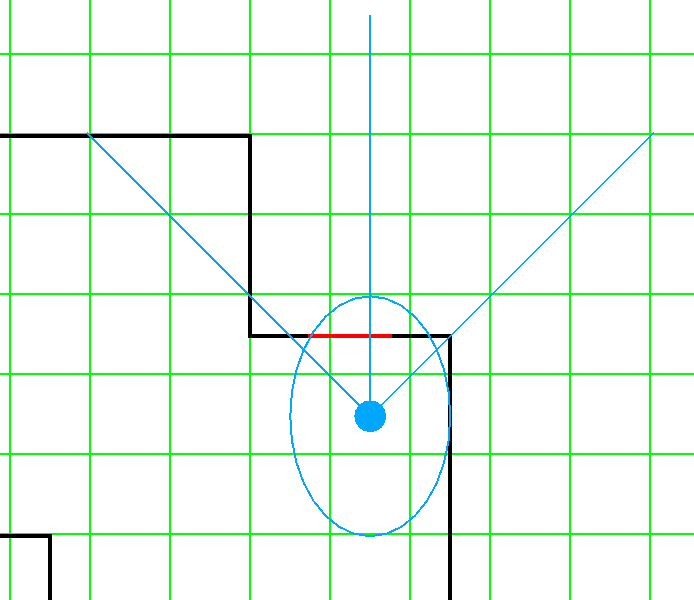
\includegraphics[scale=0.7]{./../img/covariance.png}
\caption{Repr�sentation de la covariance }
\label{cov}
\end{center}
\end{figure}

\section{Tests et R�sultats }
\subsection{Tests et r�sultats de l'impl�mentation de EKF}

\subsection{Comparaison avec le MCL}



\chapter{Occupancy Grid}







\part{Conclusions}
Cette partie finale est compos�e d'une conclusion ainsi que des propostion de recherches futures pour continuer ce m�moire. La conclusion porte aussi bien sur les notions th�orique des algorithme de localisation que sur les probl�mes pratique rencontr� au cours de m�moire. En effet, sans consid�r� la pratique il est impossible d'avoir des algorithmes de localisation de qualit�. 


\chapter{Conclusion}


Bien que les concepts globaux th�oriques des algorithmes semblent � premi�re vue simples, il s'av�re qu'impl�menter de tels algorithmes de localisation sur un robot r�el demande de r�soudre une quantit� importante de sous probl�mes.  En effet, un algorithme de localisation n'est pas un �l�ment isol�, il doit �tre incorpor� dans un tout coh�rent. Il est donc primordial d'avoir une compr�hension d'ensemble ainsi qu'une compr�hension d�taill�e de l'impl�mentation du robot. Il est �galement important de garder en t�te l'objectif du robot et d�terminer l'environnement dans lequel le robot �volue pour d�terminer l'algorithme qui correspond le mieux � ces caract�ristiques.     


\chapter{Recherches futures  }
Ce m�moire n'a fait qu'effleurer la localisation d'un robot mobile dans son environnement, ce qui n'est qu'un sous domaine de l'intelligence artificielle dans la robotique. Il y a donc un grand nombre de possibilit�s pour continuer ce m�moire. Les sections suivantes pr�sentes celle qui me semble les plus int�ressantes. 

\section{Analyse d'images}
\label{sec:Analyse d'images}
Dans ce m�moire le choix d'utiliser des codes QR a permis de simplifier la d�tection de rep�re pour l'algorithme EKF. Cependant, il n'est pas possible d'utiliser des codes QR dans toutes les situations. Il est donc important de savoir extraire des rep�res des donn�es brutes des capteurs. De nombreux algorithmes permettent d'extraire des rep�re � l'aide d'une cam�ra. Ce domaine de recherche discute des diff�rents �l�ments qui sont consid�r�s comme de bons rep�res. Par exemple, la d�tection de bord se base sur de fortes modifications de la lumi�re dans une image, l'ensemble des points o� cette forte modification de lumi�re apparait est consid�r� comme un bord. L'algorithme de Canny est un exemple d'algorithme de d�tection de bords~\cite{Canny86acomputational}.De la m�me mani�re les algorithmes de d�tection de coins tentent de d�terminer les caract�ristiques d'un coin. L'algorithme de Moravec~\cite{Moravec_1980_22} et de Harris et Stephens~\cite{Harris88acombined} sont des exemples d'algorithmes de d�tection de coins.  



 


\section{Ajout d'IA dans Lejos}


Dans un but p�dagogique, il serait int�ressant de continuer � d�velopper la librairie Lejos. Rappelons qu'elle est utilis�e par de nombreuses �coles et universit�s. Elle fournit d�j� un nombre important de classes pour manipuler un robot. Cet outil est donc parfait pour d�velopper en pratique des aspects th�oriques. Cependant, elle souffre du peu de classe permettant de d�velopper une intelligence artificielle. Il serait donc int�ressant d'impl�menter des algorithmes de localisation utilisant d'autres types de capteurs, ou bien des algorithmes de prise de d�cision pour atteindre un objectif. Ces algorithmes pourraient �tre assembl�s pour construire un tout coh�rent. De plus cette librairie est �crite en Java et avec un bon niveau de d�composition des �l�ments, elle est donc facilement r�utilisable dans d'autres projets. Elle pourrait ainsi devenir un outil semblable � ROS \footnote{ROS : \href{http://www.ros.org/}{www.ros.org} } ou MSRDS\footnote{Microsoft Robotics Developer Studio 4 : \href{https://www.microsoft.com/en-us/download/details.aspx?id=29081}{www.microsoft.com}} qui sont des outils professionnels de haute qualit� fonctionnant aussi bien sur des robots industriels que des robots de loisirs comme les drones.



% etc

% Si vous utilisez (conseillé) BibTeX pour votre bibliographie :
\bibliographystyle{acm}


\bibliography{memoire}% si le fichier BibTeX est memoire.bib

\end{document}
%%% Local Variables: 
%%% mode: latex
%%% TeX-master: t
%%% TeX-PDF-mode: t
%%% End: 
